% EGE 2027, task 3. Source IDs and URLs are kept in comments.
% Editable task bank. Append new BankTask blocks at the end of the document.
\documentclass[12pt,a4paper]{article}
\usepackage{physics-textbook}
\usepackage{graphicx,needspace}
\newif\ifShowSolutions
\ifdefined\TutorEdition
  \ShowSolutionstrue
\else
  \ShowSolutionsfalse
\fi
\newcounter{banktask}
\newcommand{\BankTask}[3]{%
  \refstepcounter{banktask}%
  \Needspace{35mm}\par\medskip\noindent\begin{minipage}{\linewidth}%
  \noindent\textbf{\thebanktask.}\quad #2\par
  \ifShowSolutions
    #3\par
    \ifdefined\TutorEdition
      \ifcsname TutorSource#1\endcsname
        \smallskip{\small\csname TutorSource#1\endcsname\par}%
      \fi
    \fi
  \fi
  \end{minipage}\par\medskip
}
\begin{document}
При расчётах принимайте $g=10\,\text{м}/\text{с}^2$, если не оговорено иное.\par\medskip



% Source B02B49: https://ege.fipi.ru/bank/questions.php?search=1&proj=BA1F39653304A5B041B656915DC36B38&qid=B02B49
\BankTask{B02B49}{
На тело, движущееся прямолинейно в инерциальной системе отсчёта, в течение $3\,\text{с}$ в направлении движения действует постоянная сила $12\,\text{Н}$. Каково увеличение импульса тела за это время? Выразите ответ в $\text{кг}\cdot\text{м}/\text{с}$.
}{
\smallskip\noindent\textbf{Решение от GPT}\par
Изменение импульса равно импульсу силы: $\Delta p=F\Delta t=12\cdot3=36\,\text{кг}\cdot\text{м}/\text{с}$. Ответ: $36\,\text{кг}\cdot\text{м}/\text{с}$.
}

% Source DC8C1F: https://ege.fipi.ru/bank/questions.php?search=1&proj=BA1F39653304A5B041B656915DC36B38&qid=DC8C1F
\BankTask{DC8C1F}{
Два тела движутся по взаимно перпендикулярным пересекающимся прямым, как показано на рисунке. Модуль импульса первого тела $p_1=8\,\text{кг}\cdot\text{м}/\text{с}$, второго тела $p_2=6\,\text{кг}\cdot\text{м}/\text{с}$. Каков модуль импульса системы этих тел после их абсолютно неупругого удара? Выразите ответ в $\text{кг}\cdot\text{м}/\text{с}$.
\begin{center}
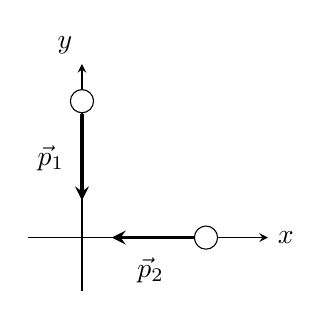
\begin{tikzpicture}[>=stealth,scale=1.05]
\draw[->] (-0.65,0)--(2.25,0) node[right] {$x$};
\draw[->] (0,-0.65)--(0,2.1) node[above left] {$y$};
\draw[fill=white] (0,1.65) circle (0.14);
\draw[very thick,->] (0,1.49)--(0,0.45);
\node[left] at (-0.1,0.96) {$\vec p_1$};
\draw[fill=white] (1.5,0) circle (0.14);
\draw[very thick,->] (1.35,0)--(0.36,0);
\node[below] at (0.83,-0.12) {$\vec p_2$};
\end{tikzpicture}
\end{center}
}{
\smallskip\noindent\textbf{Решение от GPT}\par
Импульс системы сохраняется. До удара импульсы перпендикулярны, поэтому $p=\sqrt{p_1^2+p_2^2}=\sqrt{8^2+6^2}=10\,\text{кг}\cdot\text{м}/\text{с}$. Ответ: $10\,\text{кг}\cdot\text{м}/\text{с}$.
}

% Source 225EC6: https://ege.fipi.ru/bank/questions.php?search=1&proj=BA1F39653304A5B041B656915DC36B38&qid=225EC6
\BankTask{225EC6}{
При равномерном перемещении саней по горизонтальному участку пути длиной $50\,\text{м}$ сила тяги совершает работу, величина которой равна $1000\,\text{Дж}$. Какова сила трения? Выразите ответ в ньютонах.
}{
\smallskip\noindent\textbf{Решение от GPT}\par
При равномерном движении $\Delta E_{\text{к}}=0$, поэтому $A_{\text{тяги}}+A_{\text{тр}}=0$. На горизонтальном участке $A_{\text{тр}}=-F_{\text{тр}}s$, откуда $F_{\text{тр}}=A_{\text{тяги}}/s=1000/50=20\,\text{Н}$. Ответ: $20\,\text{Н}$.
}

% Source cF941A: https://ege.fipi.ru/bank/questions.php?search=1&proj=BA1F39653304A5B041B656915DC36B38&qid=cF941A
\BankTask{cF941A}{
При подаче скорость волейбольного мяча составила $18\,\text{м}/\text{с}$. Масса мяча $280\,\text{г}$. Какова кинетическая энергия мяча? Выразите ответ в джоулях.
}{
\smallskip\noindent\textbf{Решение от GPT}\par
$m=280\,\text{г}=0{,}28\,\text{кг}$. Кинетическая энергия $E_{\text{к}}=mv^2/2=0{,}28\cdot18^2/2=45{,}36\,\text{Дж}$. Ответ: $45{,}36\,\text{Дж}$.
}

% Source ADA046: https://ege.fipi.ru/bank/questions.php?search=1&proj=BA1F39653304A5B041B656915DC36B38&qid=ADA046
\BankTask{ADA046}{
При упругой деформации, равной $3\,\text{см}$, потенциальная энергия пружины равна $6\,\text{Дж}$. На сколько изменится потенциальная энергия этой пружины при увеличении упругой деформации ещё на $3\,\text{см}$? Выразите ответ в джоулях.
}{
\smallskip\noindent\textbf{Решение от GPT}\par
$E_{\text{п}}=kx^2/2$. Деформация увеличилась вдвое, поэтому $E_2=4E_1=24\,\text{Дж}$. Изменение энергии $\Delta E=E_2-E_1=24-6=18\,\text{Дж}$. Ответ: увеличится на $18\,\text{Дж}$.
}

% Source E9E545: https://ege.fipi.ru/bank/questions.php?search=1&proj=BA1F39653304A5B041B656915DC36B38&qid=E9E545
\BankTask{E9E545}{
Шарик массой $100\,\text{г}$ падает с некоторой высоты. Начальная скорость шарика равна нулю. Его кинетическая энергия при падении на землю равна $6\,\text{Дж}$, а потеря энергии за счёт сопротивления воздуха составила $1\,\text{Дж}$. С какой высоты упал шарик? Выразите ответ в метрах.
}{
\smallskip\noindent\textbf{Решение от GPT}\par
$m=0{,}1\,\text{кг}$. При $g=10\,\text{м}/\text{с}^2$ начальная энергия $mgh=E_{\text{к}}+E_{\text{потерь}}$, откуда $h=(6+1)/(0{,}1\cdot10)=7\,\text{м}$. Ответ: $7\,\text{м}$.
}


% Source F579FA: https://ege.fipi.ru/bank/questions.php?search=1&proj=BA1F39653304A5B041B656915DC36B38&qid=F579FA
\BankTask{F579FA}{
Отношение скорости грузовика к скорости легкового автомобиля $\frac{\upsilon_1}{\upsilon_2}=\frac{1}{2}.$ Масса грузовика $m_1=3000\,\text{кг}$. Какова масса легкового автомобиля, если отношение импульса грузовика к импульсу легкового автомобиля равно $1{,}5$? Результат выразите в $\text{кг}$.
}{
\smallskip\noindent\textbf{Решение от GPT}\par
$p_1/p_2=(m_1/m_2)(v_1/v_2)$. Поэтому $m_2=m_1(v_1/v_2)/(p_1/p_2)=3000\cdot0{,}5/1{,}5=1000\,\text{кг}$.
}

% Source 72C7F7: https://ege.fipi.ru/bank/questions.php?search=1&proj=BA1F39653304A5B041B656915DC36B38&qid=72C7F7
\BankTask{72C7F7}{
Отношение импульса легкового автомобиля к импульсу мотоцикла $\frac{p_1}{p_2}=5$. Каково отношение их скоростей $\frac{\upsilon_1}{\upsilon_2},$ если отношение массы легкового автомобиля к массе мотоцикла $\frac{m_1}{m_2}=2{,}5$?
}{
\smallskip\noindent\textbf{Решение от GPT}\par
$v_1/v_2=(p_1/p_2)/(m_1/m_2)=5/2{,}5=2$.
}

% Source 568701: https://ege.fipi.ru/bank/questions.php?search=1&proj=BA1F39653304A5B041B656915DC36B38&qid=568701
\BankTask{568701}{
Тело массой $6\,\text{кг}$ движется прямолинейно со скоростью $2\,\text{м}/\text{с}$ в инерциальной системе отсчёта. На тело начала действовать постоянная тормозящая сила, равная по модулю $4\,\text{Н}$. Сколько времени пройдёт до момента остановки тела? Результат выразите в $\text{с}$.
}{
\smallskip\noindent\textbf{Решение от GPT}\par
При торможении $Ft=mv_0$. Время до остановки $t=6\cdot2/4=3\,\text{с}$.
}

% Source 8CAE7B: https://ege.fipi.ru/bank/questions.php?search=1&proj=BA1F39653304A5B041B656915DC36B38&qid=8CAE7B
\BankTask{8CAE7B}{
Тело движется в инерциальной системе отсчёта по прямой в одном направлении под действием постоянной силы величиной $5\,\text{Н}$. За $4\,\text{с}$ импульс тела увеличился и стал равен $35\,\text{кг}\cdot\text{м}/\text{с}$. Чему был равен первоначальный импульс тела? Результат выразите в $\text{кг}\cdot\text{м}/\text{с}$.
}{
\smallskip\noindent\textbf{Решение от GPT}\par
$p-p_0=Ft$, откуда $p_0=35-5\cdot4=15\,\text{кг}\cdot\text{м}/\text{с}$.
}

% Source 107015: https://ege.fipi.ru/bank/questions.php?search=1&proj=BA1F39653304A5B041B656915DC36B38&qid=107015
\BankTask{107015}{
В инерциальной системе отсчёта тело движется по прямой в одном направлении под действием постоянной силы. За $2\,\text{с}$ импульс тела изменился на $8\,\text{кг}\cdot\text{м}/\text{с}$. Каков модуль силы? Результат выразите в $\text{Н}$.
}{
\smallskip\noindent\textbf{Решение от GPT}\par
$F=\Delta p/\Delta t=8/2=4\,\text{Н}$.
}

% Source 7998DB: https://ege.fipi.ru/bank/questions.php?search=1&proj=BA1F39653304A5B041B656915DC36B38&qid=7998DB
\BankTask{7998DB}{
Два тела движутся с одинаковой скоростью. Кинетическая энергия первого тела в $4$ раза меньше кинетической энергии второго тела. Определите отношение $\frac{m_1}{m_2}$ масс тел.
}{
\smallskip\noindent\textbf{Решение от GPT}\par
При одинаковых скоростях $E_{\text{к}1}/E_{\text{к}2}=m_1/m_2=1/4=0{,}25$.
}

% Source 354CDE: https://ege.fipi.ru/bank/questions.php?search=1&proj=BA1F39653304A5B041B656915DC36B38&qid=354CDE
\BankTask{354CDE}{
Тело массой $0{,}1\,\text{кг}$ вращается в горизонтальной плоскости на нити длиной
$1\,\text{м}$. Чему равна работа силы тяжести за один оборот вращения тела? Результат выразите в $\text{Дж}$.
}{
\smallskip\noindent\textbf{Решение от GPT}\par
При движении в горизонтальной плоскости $\Delta h=0$. Работа силы тяжести $A=-mg\Delta h=0\,\text{Дж}$.
}

% Source BD865C: https://ege.fipi.ru/bank/questions.php?search=1&proj=BA1F39653304A5B041B656915DC36B38&qid=BD865C
\BankTask{BD865C}{
Шайба соскальзывает по гладкой наклонной плоскости из состояния покоя
с высоты $80\,\text{см}$. Какова максимальная скорость шайбы у основания наклонной плоскости? Сопротивлением воздуха пренебречь. Результат выразите в $\text{м}/\text{с}$.
}{
\smallskip\noindent\textbf{Решение от GPT}\par
$mgh=mv^2/2$. При $h=0{,}8\,\text{м}$ получаем $v=\sqrt{2gh}=\sqrt{2\cdot10\cdot0{,}8}=4\,\text{м}/\text{с}$.
}

% Source 1C4DA4: https://ege.fipi.ru/bank/questions.php?search=1&proj=BA1F39653304A5B041B656915DC36B38&qid=1C4DA4
\BankTask{1C4DA4}{
Первая пружина имеет жёсткость $20\,\text{Н}/\text{м}$, вторая — $40\,\text{Н}/\text{м}$. Первая растянута на $2\,\text{см}$, вторая — на $1\,\text{см}$. Чему равно отношение потенциальной энергии второй пружины к потенциальной энергии первой $\frac{E_2}{E_1}?$
}{
\smallskip\noindent\textbf{Решение от GPT}\par
$E_2/E_1=k_2x_2^2/(k_1x_1^2)=(40/20)(1/2)^2=0{,}5$.
}

% Source 1F9FAE: https://ege.fipi.ru/bank/questions.php?search=1&proj=BA1F39653304A5B041B656915DC36B38&qid=1F9FAE
\BankTask{1F9FAE}{
Жёсткость пружины равна $7500\,\text{Н}/\text{м}$. Какова энергия упругой деформации этой пружины при её растяжении на $4\,\text{см}$? Результат выразите в $\text{Дж}$.
}{
\smallskip\noindent\textbf{Решение от GPT}\par
$x=0{,}04\,\text{м}$. Энергия $E=kx^2/2=7500\cdot0{,}04^2/2=6\,\text{Дж}$.
}

% Source B41DCC: https://ege.fipi.ru/bank/questions.php?search=1&proj=BA1F39653304A5B041B656915DC36B38&qid=B41DCC
\BankTask{B41DCC}{
Легковой автомобиль и грузовик движутся по горизонтальному мосту. Масса грузовика $m=4500\,\text{кг}$. Какова масса легкового автомобиля, если отношение потенциальной энергии грузовика к потенциальной энергии легкового автомобиля относительно уровня воды в реке равно $3$? Результат выразите в $\text{кг}$.
}{
\smallskip\noindent\textbf{Решение от GPT}\par
На одном мосту высота над водой одинакова: $E_{\text{п}1}/E_{\text{п}2}=m_1/m_2$. Тогда $m_2=4500/3=1500\,\text{кг}$.
}

% Source 2785A3: https://ege.fipi.ru/bank/questions.php?search=1&proj=BA1F39653304A5B041B656915DC36B38&qid=2785A3
\BankTask{2785A3}{
Мальчик на санках спустился с ледяной горы высотой $10\,\text{м}$ и проехал по горизонтали до остановки $50\,\text{м}$. Чему равен коэффициент трения санок по горизонтальной поверхности? Считать, что по склону горы санки скользили без трения.
}{
\smallskip\noindent\textbf{Решение от GPT}\par
На склоне $E_{\text{к}}=mgh$, на горизонтальном участке $\mu mgs=mgh$. Поэтому $\mu=h/s=10/50=0{,}2$.
}

% Source 8CED26: https://ege.fipi.ru/bank/questions.php?search=1&proj=BA1F39653304A5B041B656915DC36B38&qid=8CED26
\BankTask{8CED26}{
Сталкиваются и слипаются два разных по массе пластилиновых шарика, причём векторы их скоростей непосредственно перед столкновением направлены навстречу друг другу и одинаковы по модулю: $\upsilon_{1}=\upsilon_{2}=1\,\text{м}/\text{с}$. Во сколько раз масса тяжёлого шарика больше, чем лёгкого, если сразу после столкновения их скорость стала равной (по модулю) $0{,}5\,\text{м}/\text{с}$?
}{
\smallskip\noindent\textbf{Решение от GPT}\par
Положительное направление выберем по движению тяжёлого шарика. По сохранению импульса $(M-m)\cdot1=(M+m)\cdot0{,}5$. Отсюда $M/m=3$.
}

% Source B34015: https://ege.fipi.ru/bank/questions.php?search=1&proj=BA1F39653304A5B041B656915DC36B38&qid=B34015
\BankTask{B34015}{
Автомобиль с выключенным двигателем сняли со стояночного тормоза, и он покатился под уклон, составляющий угол $30\,{}^\circ$ с горизонтом. В начале горизонтального участка дороги, который следует за спуском, его скорость составляет $10\,\text{м}/\text{с}$. Какое расстояние автомобиль проезжает по склону? Трением пренебречь. Результат выразите в $\text{м}$.
}{
\smallskip\noindent\textbf{Решение от GPT}\par
$mgs\sin30^\circ=mv^2/2$. Тогда $s=v^2/(2g\sin30^\circ)=100/(2\cdot10\cdot0{,}5)=10\,\text{м}$.
}

\end{document}
